\chapter{Implementacja}
\begin{figure}[h]
 \centering
 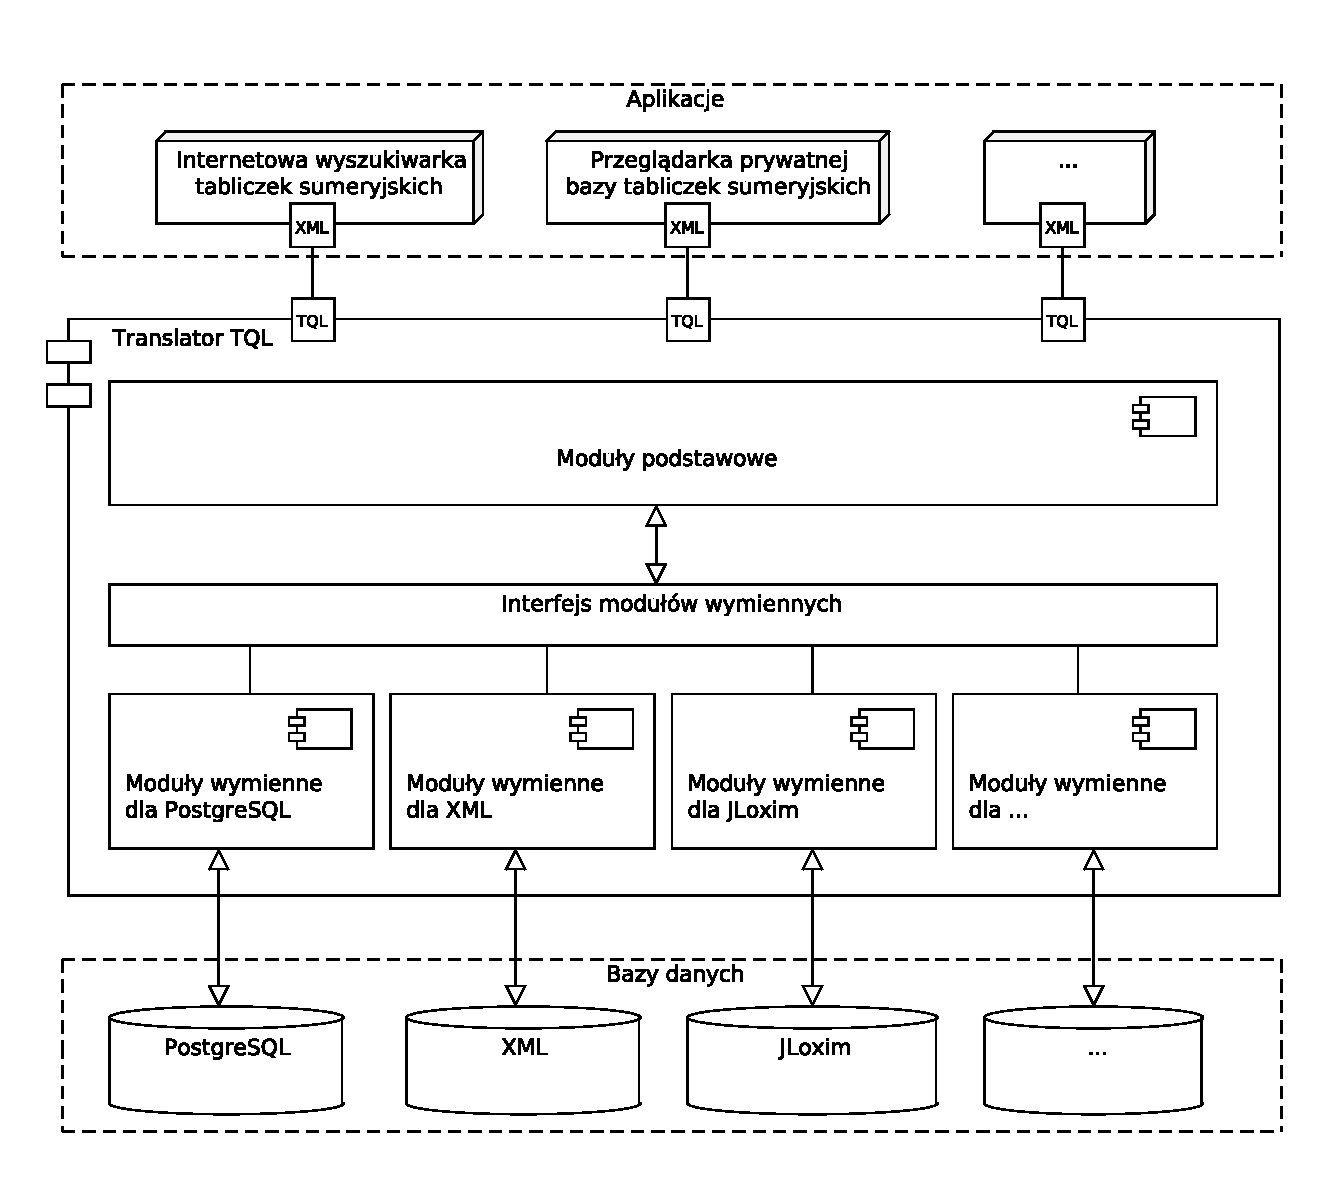
\includegraphics[width=500px,bb=0 0 608 517]{../diagramy/struktura2.pdf}
 % struktura.pdf: 608x517 pixel, 72dpi, 21.45x18.24 cm, bb=0 0 608 517
 \caption{Struktura systemu korzystającego z translatora}
\end{figure}

\begin{figure}
 \centering
 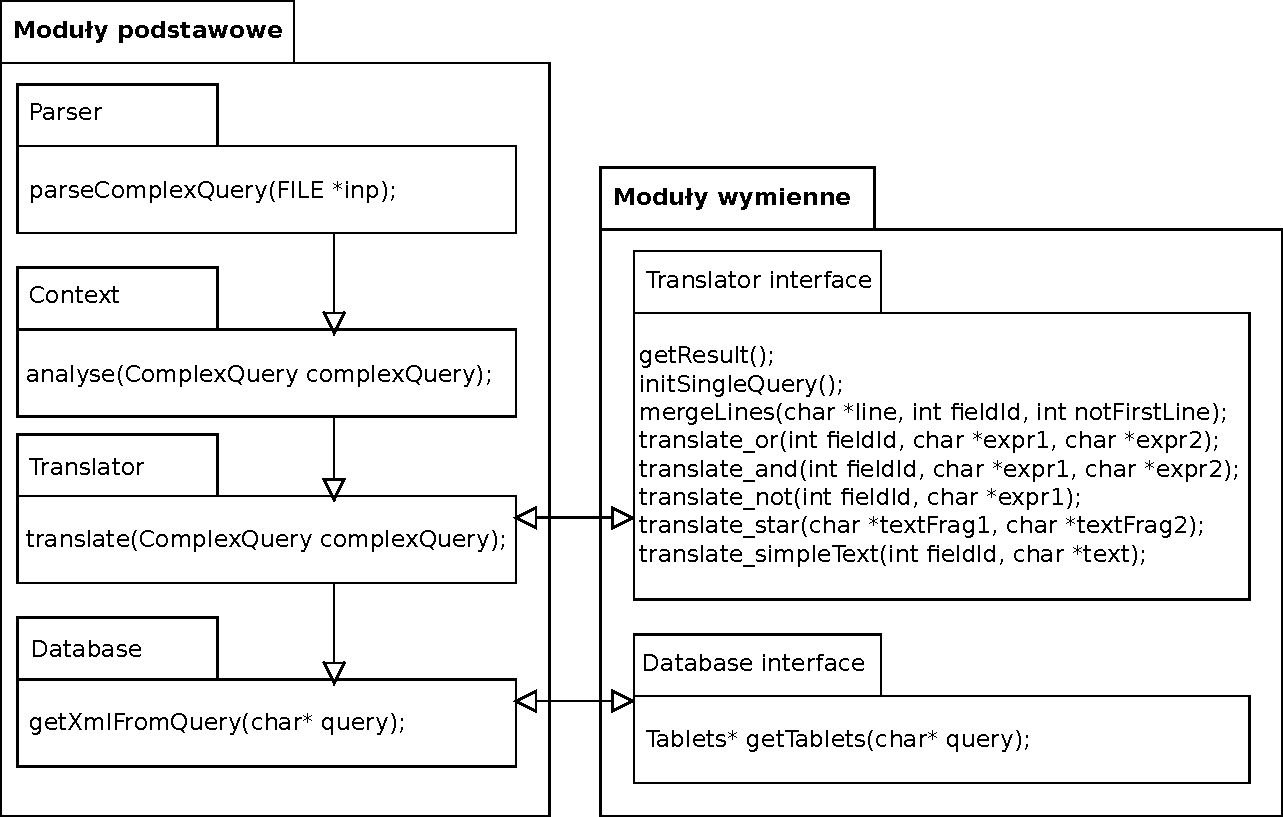
\includegraphics[width=500px,bb=0 0 585 300]{../diagramy/pakiety.pdf}
 % pakiety.pdf: 585x300 pixel, 72dpi, 20.64x10.58 cm, bb=0 0 585 300
 \caption{Podział programu na moduły}
\end{figure}
Jednym z głównych założeń języka TQL jest niezależność od struktury danych.
W związku z tym istotną cechą translatora jest możliwość dostosowania do współpracy z różnymi bazami danych.
%Jednym z głównych wymagań postawionych przed translatorem, żeby można było podłączyć różne bazy danych.
 Wynikiem tego jest podział translatora na 2 rodzaje modułów:
\begin{enumerate}
 \item \textbf{Podstawowe} -- niezależne od struktury danych i zajmujące się głównie parsowaniem i analizą składniową zapytania.
 \item \textbf{Wymienne} -- zależne od struktury danych, tłumaczące zapytanie TQL na język odpowiedni dla używanej bazy danych
i wywołujące je.
\end{enumerate}
 Wybór modułu wymiennego odbywa się na poziomie kompilacji. 
%Bez względu na wybór modułu wymiennego interfejs całego translatora jest taki sam we wszystkich instancjach.


\section{Moduły podstawowe}

\subsection{Parser}
Parser został utworzony za pomocą narzędzia BNFC. Następnie zostały w nim wprowadzone modyfikacje:
\begin{itemize}
\item poprawienie nazw stałych oznaczających symbole na bardziej intuicyjne,
\item dodanie tablicy symboli,
\item usunięcie niepotrzebnych funkcji z interfejsu,
\item uporządkowanie kodu.
\end{itemize}
Moduł ten parsuje zapytanie w języku TQL, tworząc drzewo struktury składniowej, które jest zdefiniowane w pliku pomocniczym Absyn.h.
Na parser składają się następujące pliki:
\begin{itemize}
 \item Parser.c
 \item Parser.h
 \item TQL.y % tłumaczony na Parser.c
 \item TQL.l % tłumaczony na Lexer.c
\end{itemize}

\subsection{Analizator kontekstowy}
Moduł analizuje drzewo struktury składniowej w następujący sposób:
\begin{itemize}
 \item sprawdza, czy podano prawidłowe nazwy pól,  %to co jest po lewej w linii zapytania jest nazwą pola.
\item upraszcza drzewo - z wywołania zapytania (wywołanie \textit{search in}) tworzy zapytanie proste.
\end{itemize}
Składa się z następujących plików:
\begin{itemize}
 \item Context.c
 \item Context.h
\end{itemize}

\subsection{Translator}
Zadaniem translatora jest przetłumaczenie drzewa składni abstrakcyjnej na zapytanie w docelowym języku. 
Składa się z następujących plików:
\begin {itemize}
 \item Translator.c
 \item Translator.h
 \item Translator\_config.h (interfejs modułu translatora zależnego od bazy danych)
 %\item Translator\_config.c (implementacja interfejsu z Translator\_config.h, zależny od wyboru bazy danych itp)
\end {itemize}

Tłumaczenie poszczególnych elementów drzewa zależy od implementacji interfejsu zawartego w pliku Translator\_config.h. 
Funkcja translate() przechodzi całą strukturę drzewa, wywołując w razie potrzeby odpowiednie funkcje z Translator\_config.
Następnie pobiera przetłumaczone zapytanie za pomocą funkcji getResult(), aby przekazać je do modułu bazy.

\subsection{Baza}
Moduł bazy jest odpowiedzialny za wywołanie przetłumaczonego zapytania i przekazanie wyniku w określonej formie - jako XML.
Składa się z następujących plików:
\begin {itemize}
 \item Database.c
 \item Database.h
 \item Database\_config.h (interfejs modułu bazy zależnego od bazy danych)
% \item Database\_config.c (implementacja interfejsu z Database\_conf.h, zależny od wyboru bazy danych itp)
\end {itemize}

Wywołuje funkcję getTablets() z Database\_config.h, jako parametr podając przetłumaczoną treść zapytania. 
Funkcja ta zwraca strukturę danych Tablets, wypełnioną informacjami o wyszukanych tabliczkach.
Następnie na podstawie otrzymanej struktury tworzony jest dokument XML.
\newline
Definicja struktury Tablets:
\begin{verbatim}
typedef struct{    
    char* id;
    char* id_cdli;
    char* publication;
    char* measurements;
    char* year;
    char* provenience;
    char* period;
    char* genre;
    char* subgenre;
    char* collection;
    char* text;
    Tags *tags; // specjalnie oznaczone miejsca w tekscie
                // (w pierwszej wersji frazy wyszukiwania)
} Tablet;

typedef struct{
    int size;
    Tablet *tabs;
} Tablets;
\end{verbatim}

%//miejsca gdzie w tekście są wyniki wyszukiwania

%Wszystkie niezbędne informacje powinny się znajdować w bazie danych.

\subsection{Pliki pomocnicze}
Definicje struktur danych (wygenerowane za pomocą BNFC, następnie uproszczone):
\begin{itemize}
 \item Absyn.c
\item Absyn.h
\end{itemize}
Tablica symboli:
\begin{itemize}
 \item Symbols.c
\item Symbols.h
\end{itemize}
Obsługa błędów:
\begin{itemize}
 \item Err.c
\item Err.h
\end{itemize}
Moduł do dzielenia tekstu względem separatora, pobrany z internetu \cite{cexplode}:
\begin{itemize}
 \item Cexplode.c
 \item Cexplode.h
\end{itemize}


\section{Moduły wymienne}
Pliki zależne od wyboru konkretnej bazy danych to:
\begin{itemize}
 \item Translator\_config.c - dla modułu translatora
\item Database\_config.c - dla modułu bazy
\end{itemize}
Ich interfejsy są wspólne dla wszystkich baz danych.


\section{Baza PostgreSQL}
\subsection{Diagram encji}
\begin{figure}[h]
 \centering
 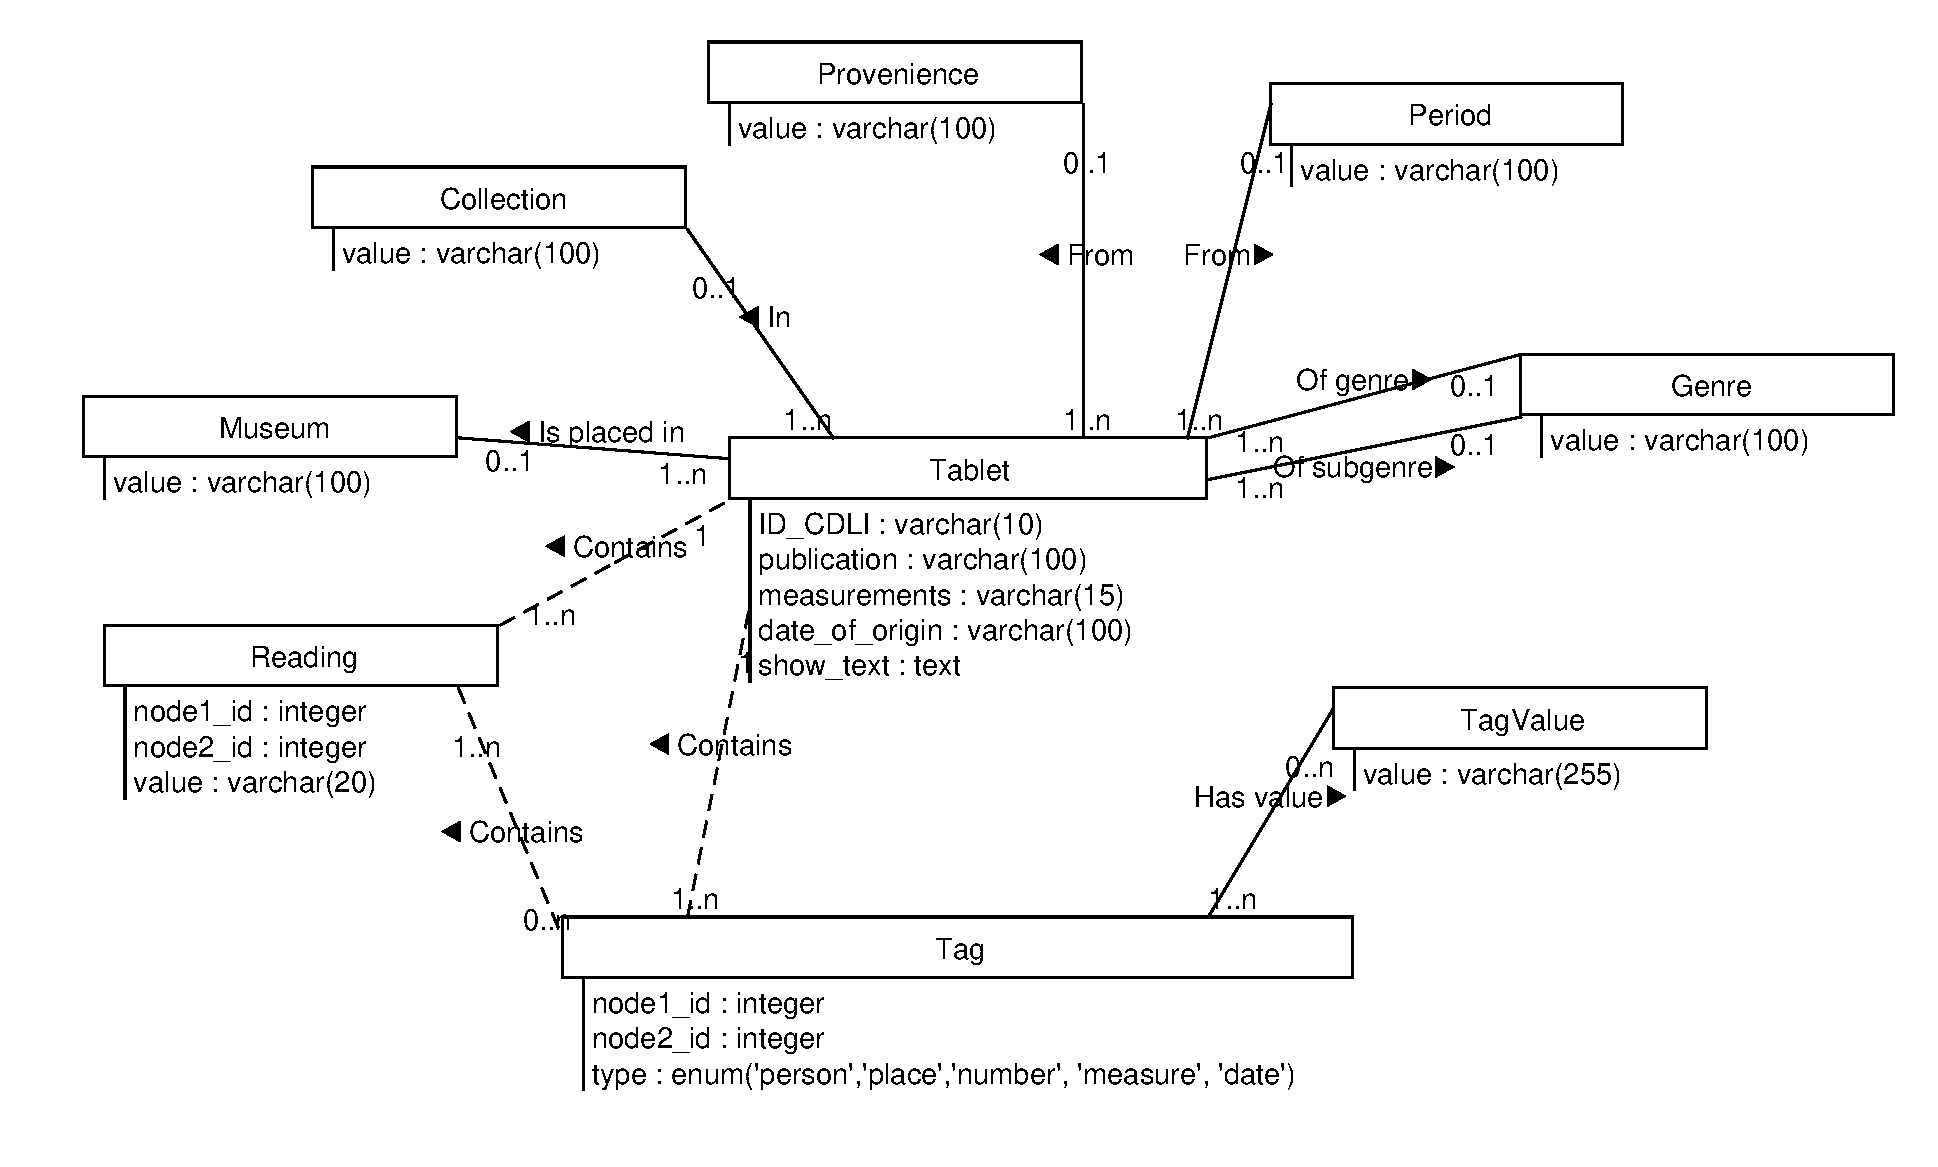
\includegraphics[width=500px,bb=0 0 930 560]{../diagramy/diagram-encji-maly.pdf}
 % diagram-encji-maly.pdf: 930x560 pixel, 72dpi, 32.81x19.76 cm, bb=0 0 930 560
 \caption{Diagram encji}
\end{figure}
Jednym z problemów przy projektowaniu bazy danych był wybór takiej reprezentacji treści tabliczki, 
żeby efektywnie wyszukiwać zarówno treść konkretnej tabliczki jak i tabliczki, których treść spełnia podane kryteria
 (wg odczytów lub zapisu klinowego).

W przypadku pierwszego problemu jako rozwiązanie narzuca się przechowywanie treści
jako otwarty tekst.
Natomiast najlepszym rozwiązaniem drugiego jest reprezentacja treści tabliczki
w formie grafu, którego krawędziami są odczyty i kliny (zgodnie z pomysłem dr Wojciecha Jaworskiego\cite[s.13-24]{jaworski}).
Zdecydowałyśmy się na połączenie obu sposobów. Odczyty oraz kliny przechowujemy w tabelach Reading i Cuneiform, 
natomiast otwarty tekst w kolumnie show\_text tabeli Tablet. 
% TODO: chyba trochę lepiej
Dzięki temu rozwiązaniu, szukając tabliczki zawierającej podane odczyty (lub kliny) korzystamy z reprezentacji
grafowej w tabelce Reading (lub Cuneiform).
Natomiast zawsze korzystamy z reprezentacji otwartym tekstem w tabelce Tablet w celu wyświetlenia treści tabliczki.
% Aby zapewnić możliwość odwzorowania treści tabliczki między reprezentacjami, węzły są liczbami postaci:
Kiedy więc wyszukujemy w tabelce Reading (lub Cuneiform) musimy być wstanie powiązać znalezione odczyty (kliny) 
z całą treścią tabliczki w tabeli Tablet. Osiągamy to zapisując węzły w grafie w postaci:
\begin{verbatim}
 <numer węzła w tabliczce> * 1 000 000 + <id tabliczki>
\end{verbatim}
gdzie numer węzła w tabliczce to numer kolejnego słowa (słowa są oddzielone spacjami i końcem linii) pomnożone przez 10 
(żeby umożliwić wstawienie kilku węzłów w jednym słowie np. pozwolić na przetłumaczenie jednego słowa na sekwencję trzech klinów). 


Przerywane linie na diagramie encji oznaczają opisany powyżej związek pomiędzy id węzła (node1\_id i node2\_id) 
a id tabliczki (Tablet.id).

% relacja
% Stąd wzięły się przerywane linie na diagramie encji - nie ma bezpośredniego klucza obcego w tabeli Reading (czy Tag) do Tablet, 
% jednak związek istnieje. Taki sposób przechowywania informacji o treści tabliczki umożliwia sprawniejsze wyszukiwanie nie tylko
% po odczytach (pozwala pomijać linie z uszkodzeniami) ale także w przyszłości ułatwia zaimplementowanie wyszukiwania po klinach,
% po tagach itp.
% Poza sprawnym
%  wyszukiwaniem ułatwia to rozszerzenie programu o możliwość wyszukiwania po klinach - po dodaniu tabeli Cuneiform.

 

\subsection{Translator\_postgres}
Tłumaczy otrzymane fragmenty drzewa struktury zapytania na język SQL. Przetłumaczone fragmenty zbiera do buforów 
(\textit{select}, \textit{from}, \textit{where}), które następnie odpowiednio łączy.
Każde proste zapytanie TQL jest tłumaczone na pojedyncze zapytanie SQL. Tłumaczenie kilku prostych zapytań
łączone jest za pomocą UNION.

\subsubsection{Stałe fragmenty zapytania}
Tłumaczenie prostego zapytania zaczyna się od inicjalizacji buforów przechowujących poszczególne części wynikowego SQL-a.\\
\textit{select} jest inicjowany na 
\begin{verbatim}
SELECT t.id, t.id_cdli, t.publication, t.measurements, t.origin_date, 
       p.value as provenience, pd.value as period,
       g1.value as genre, g2.value as subgenre, 
       c.value as collection, t.text
\end{verbatim}
\textit{from} jest inicjowany
\begin{verbatim}
FROM tablet t
  LEFT JOIN provenience p ON p.id = t.provenience_id
  LEFT JOIN collection c ON c.id = t.collection_id
  LEFT JOIN genre g1 ON g1.id = t.genre_id
  LEFT JOIN genre g2 ON g2.id = t.subgenre_id
  LEFT JOIN period pd ON pd.id = t.period_id
\end{verbatim}
\textit{where} początkowo zawiera pusty ciąg znaków.



\subsubsection{Tłumaczenie zapytań o atrybuty tabliczki}
Poniższe tłumaczenia są dodawane do bufora \textit{where} i łączone za pomocą AND.
\begin{longtable}{|p{3in}|p{3in}|}
\hline
{\bf Konstrukcja} & {\bf Tłumaczenie na SQL}\\
\hline
\endhead
provenience: wartosc & \begin{verbatim}p.value LIKE 'wartosc'\end{verbatim}
\\
\hline
publication: wartosc & 
\begin{verbatim}
t.publication LIKE 'wartosc'
\end{verbatim}
\\
\hline
period: wartosc & 
\begin{verbatim}
pd.value LIKE 'wartosc'
\end{verbatim}
\\
\hline
year: wartosc & 
\begin{verbatim}
t.origin_date LIKE 'wartosc'
\end{verbatim}
\\
\hline
genre: wartosc & 
\begin{verbatim}
   g1.value LIKE 'wartosc' 
OR g2.value LIKE 'wartosc'
\end{verbatim}
\\
\hline
cdli\_id: wartosc & 
\begin{verbatim}
t.cdli_id LIKE 'wartosc'
\end{verbatim}
\\
\hline
museum: wartosc & 
\begin{verbatim}
t.museum LIKE 'wartosc'
\end{verbatim}
\\
\hline
collection: wartosc & 
\begin{verbatim}
c.value LIKE 'wartosc'
\end{verbatim}
\\
\hline
\end{longtable}

\textbf{Tłumaczenie operatorów:}
\begin{longtable}{|p{1in}|p{1in}|}
\hline
{\bf Operator} & {\bf Tłumaczenie}\\
\hline
\endhead
/ & OR\\ 
\hline
-- & NOT\\ 
\hline
+ & AND\\ 
\hline
* & \%  \\ 
\hline
\end{longtable}


\subsubsection{Tłumaczenie zapytań o treść tabliczki}
Przy tłumaczeniu zapytań o treść tabliczki
korzystamy z przedstawienia treści tabliczki w formie grafu.

Pojawienie się wyszukiwania po treści tabliczki niesie za sobą konieczność dodania do bufora \textit{from}:
\begin{verbatim}
INNER JOIN (
  <wynikowe zapytanie o treść tablczki>
) AS sequence ON sequence.id_tab = t.id
\end{verbatim}

natomiast do \textit{select} dodajemy:
\begin{verbatim}
, sequence.nodes as nodes
\end{verbatim}

gdzie $<$wynikowe zapytanie o treść tablczki$>$ to kombinacja zapytań typu:
\begin{verbatim}
  SELECT 
    id_tab, 
    CAST(array_accum(nodes) as TEXT) as nodes, 
    COUNT(DISTINCT id_seq) AS seq, 
    <id_sekw> AS id_seq
  FROM (
    SELECT
      t1.node1_id % 1000000 AS id_tab,
      '{' || t1.node1_id || ',' || t<dl_sekw>.node2_id || '}' AS nodes,
      1 AS id_seq
    FROM
      <nazwa_tabeli> t1
      LEFT JOIN <nazwa_tabeli> t2 ON (t2.node1 = t1.node2)
      LEFT JOIN <nazwa_tabeli> t3 ON (t3.node1 = t2.node2)
      ...
      LEFT JOIN <nazwa_tabeli> t<dl_sekw> ON (t<dl_sekw>.node1 = t<dl_sekw-1>.node2)
   WHERE
      t1.value LIKE '<sekw[1]>'
     AND
      t2.value LIKE '<sekw[2]>'
    AND
      t3.value LIKE '<sekw[3]>'
    AND
      ...
    AND
      t<dl_sekw>.value LIKE '<sekw[<dl_sekw>]>'
   ) AS a 
  GROUP BY id_tab
\end{verbatim}
Zmienne użyte w powyższym pseudo-kodzie:
\begin{description}
 \item[id\_sekw] - kolejny numer sekwencji (przydatny przy bardziej skomplikowanym zapytaniu - do rozróżniania podzapytań)
 \item[dl\_sekw] - ilość słów składających się na wyszukiwaną sekwencję
 \item[sekw] - tablica zawierająca słowa składające się na wyszukiwaną sekwencję
\item[nazwa\_tabeli] - nazwa tabeli, w której wyszukujemy (Reading lub Cuneiform)
 \end{description}

\begin{longtable}{|p{1in}|p{4.5in}|}
\hline
{\bf Operator} & {\bf Tłumaczenie}\\
\hline
\endhead
/ & 
\begin{verbatim}
SELECT 
  id_tab, 
  CAST(array_accum(nodes) as TEXT) as nodes, 
  COUNT(DISTINCT id_seq) as seq,
  <id_sekw> as id_seq
FROM 
(
  <zapytanie1>
  UNION
  <zapytanie2>
)
as c
GROUP BY id_tab
\end{verbatim}
\\ 
\hline
+ &
\begin{verbatim}
SELECT * FROM
 (SELECT id_tab, 
         CAST(array_accum(nodes) as TEXT) as nodes, 
         COUNT(DISTINCT id_seq) as seq, 
         <id_sekw> as id_seq
  FROM
    (<zapytanie1>
    UNION
    <zapytanie2>)
  as c 
  GROUP BY id_tab
 ) as b
WHERE b.seq=2 
\end{verbatim}
\\ 
\hline
-- & 
\begin{verbatim}
SELECT 
  id_tab, 
  '' as nodes, 
  0 as seq,
  <id_sekw> as id_seq
FROM
(
 (SELECT id as id_tab from tablet)
 EXCEPT
 (SELECT id_tab from
    <zapytanie_negowane> as a
 )   
) as b
\end{verbatim}
\\ 
\hline
* & \%  \\ 
\hline
\end{longtable}


\subsection{Database\_postgres}

Odpowiada za wywołanie zapytania w konkretnej bazie i zapisanie wyniku do struktury Tablets.
 Korzysta z pliku database.conf, który zawiera dane dostępu do bazy (nazwa bazy, host, port, użytkownik, hasło)
oraz biblioteki libpq-fe.h do PostgreSQL.

\subsection{Baza XML}

\subsubsection{Schemat dokumentu}

\begin{figure}[h]
 \centering
 \subfigure[element text]{
 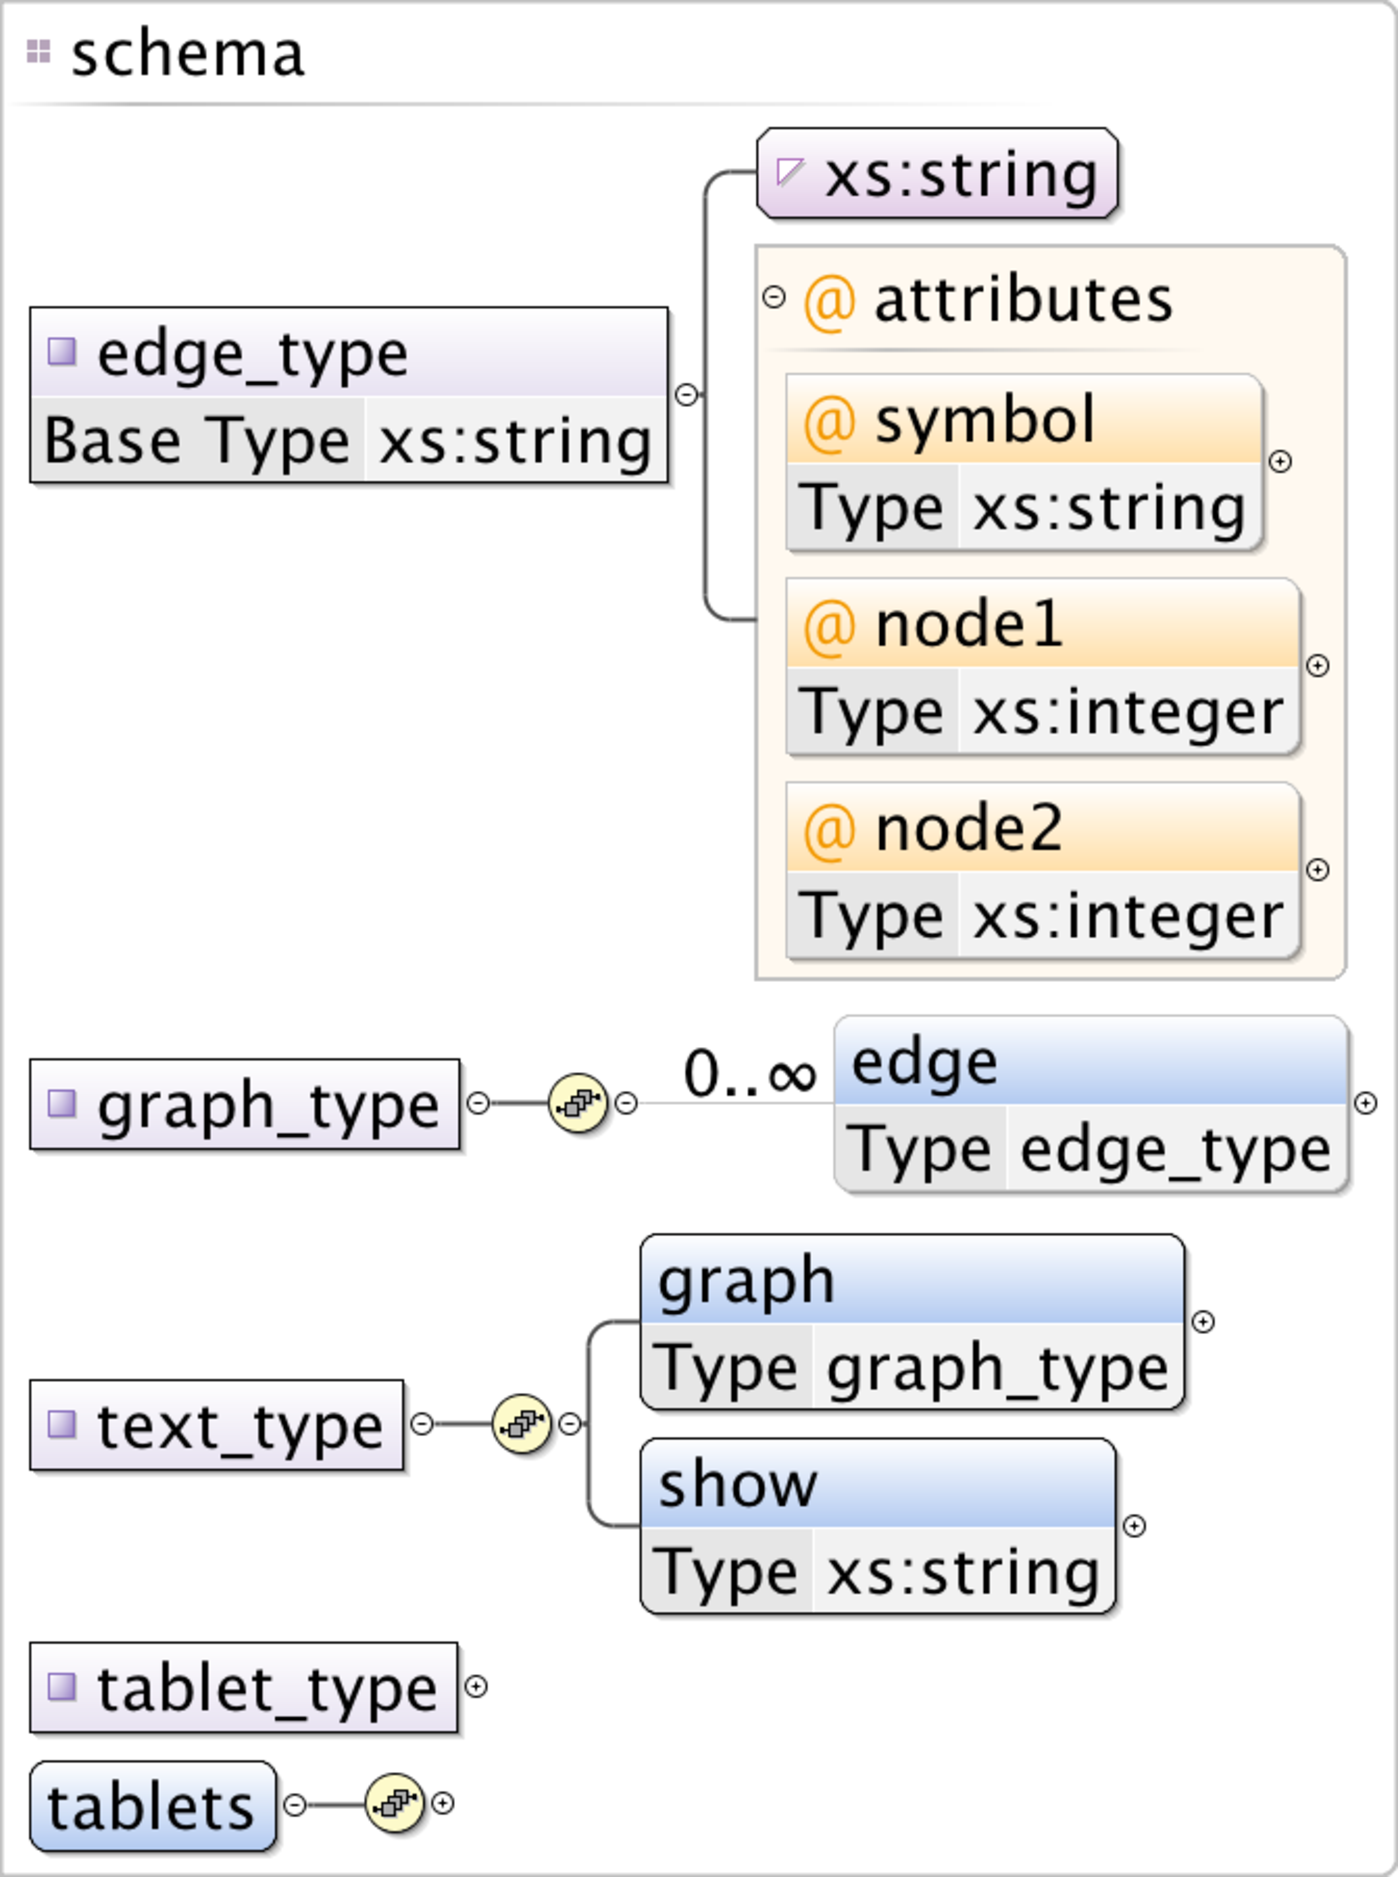
\includegraphics[width=120px]{../diagramy/schema_text.pdf}
 }
   \subfigure[element tablet]{
  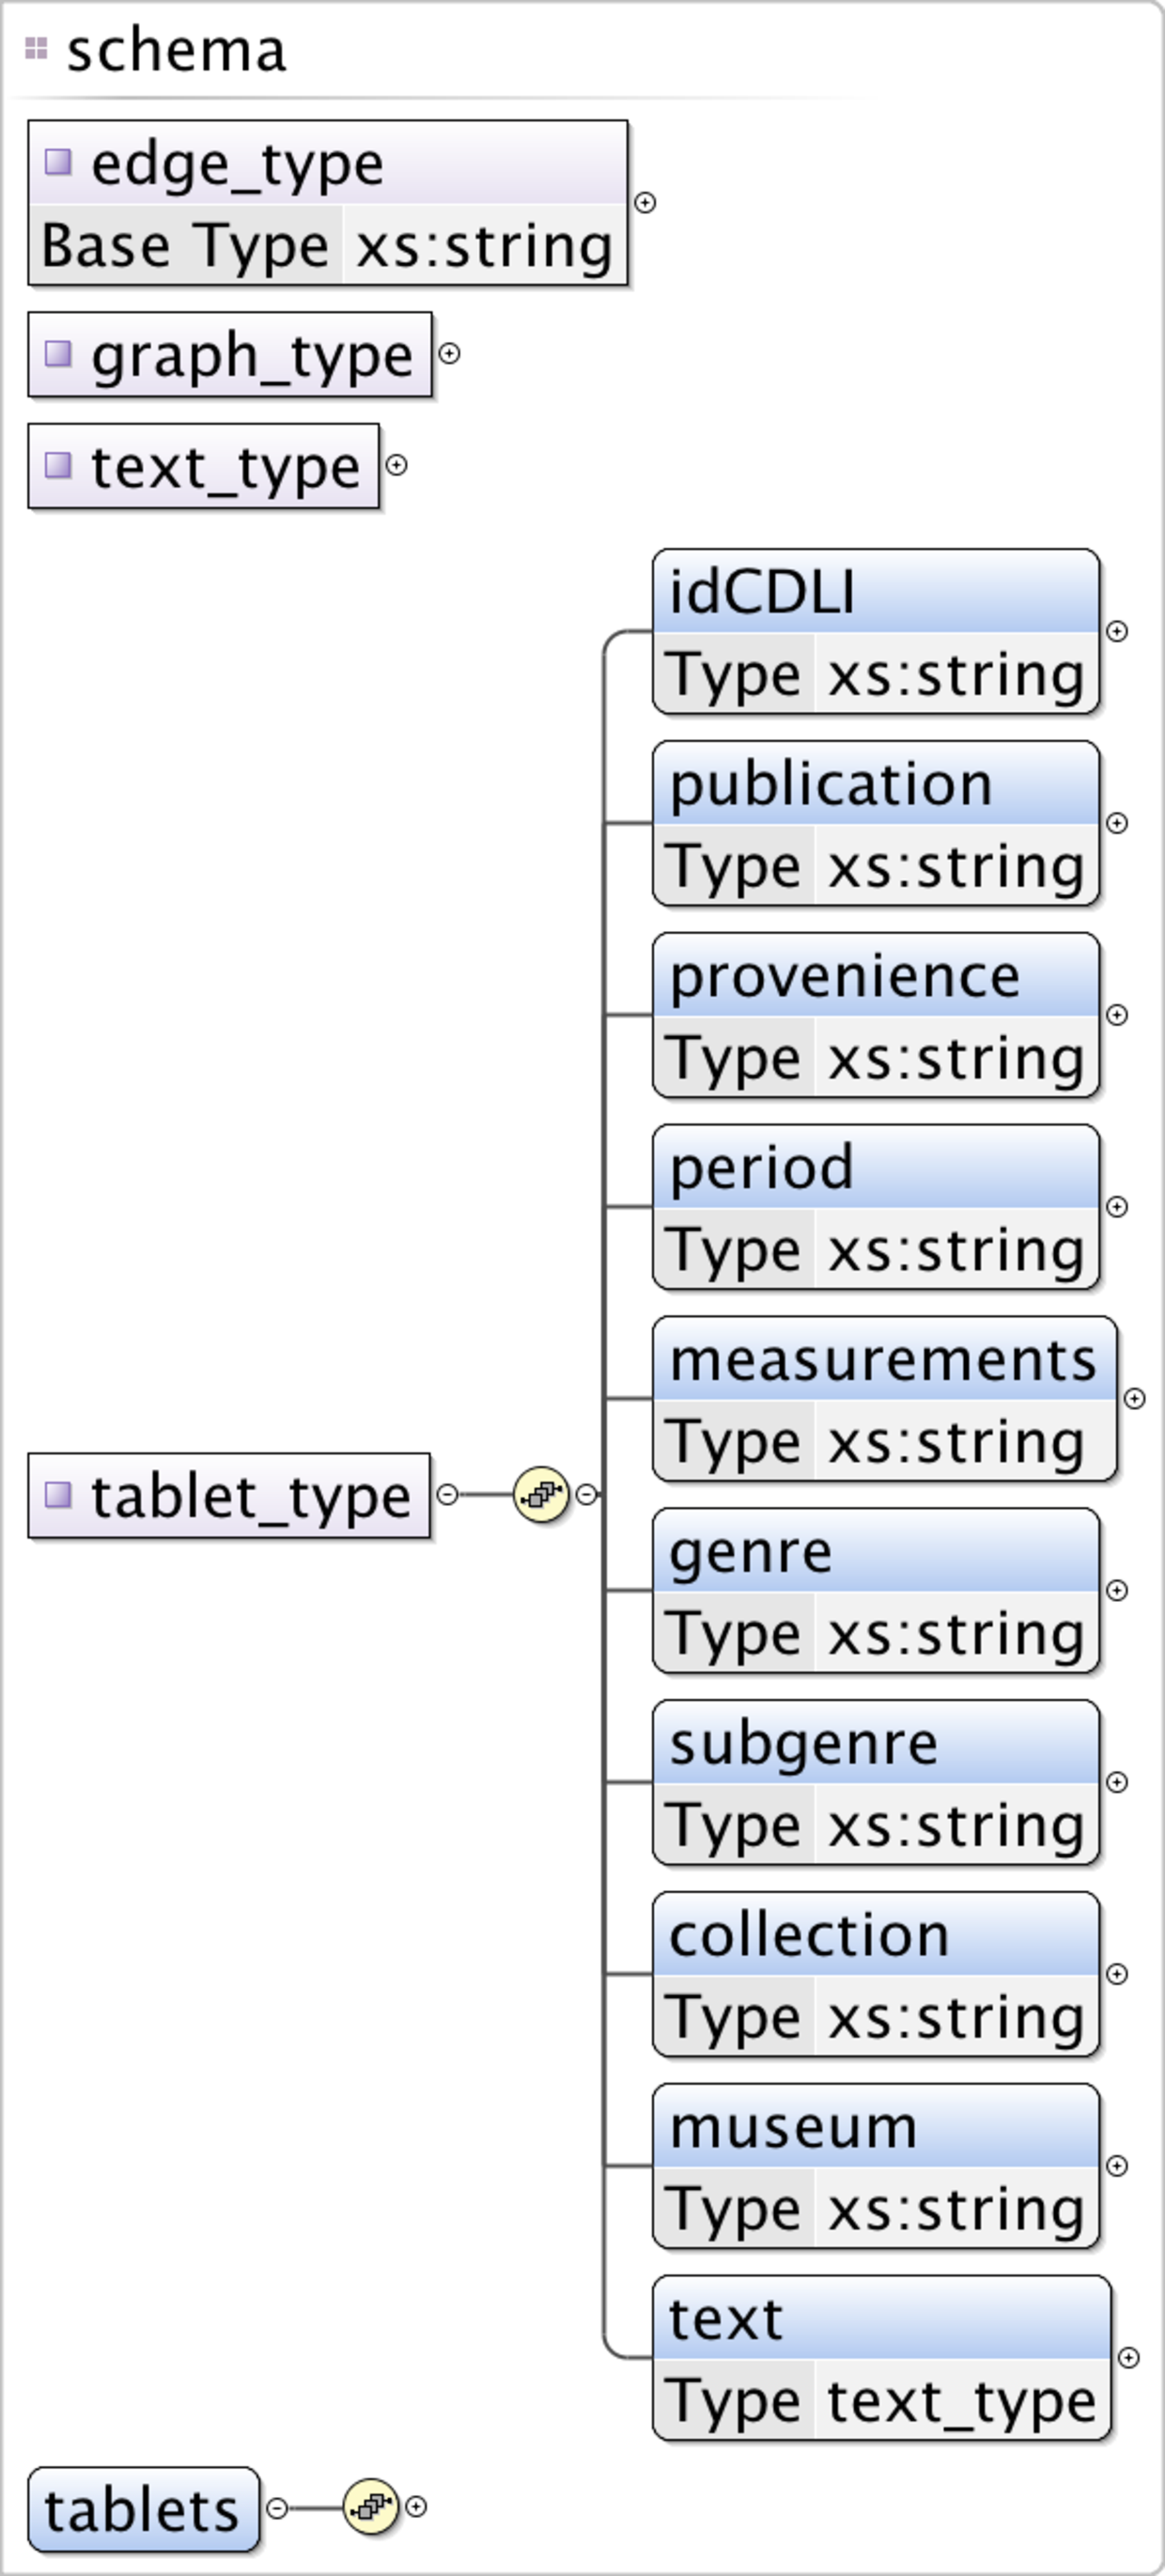
\includegraphics[width=120px]{../diagramy/schema_tablet.pdf}
 }
 \subfigure[element tablets]{
  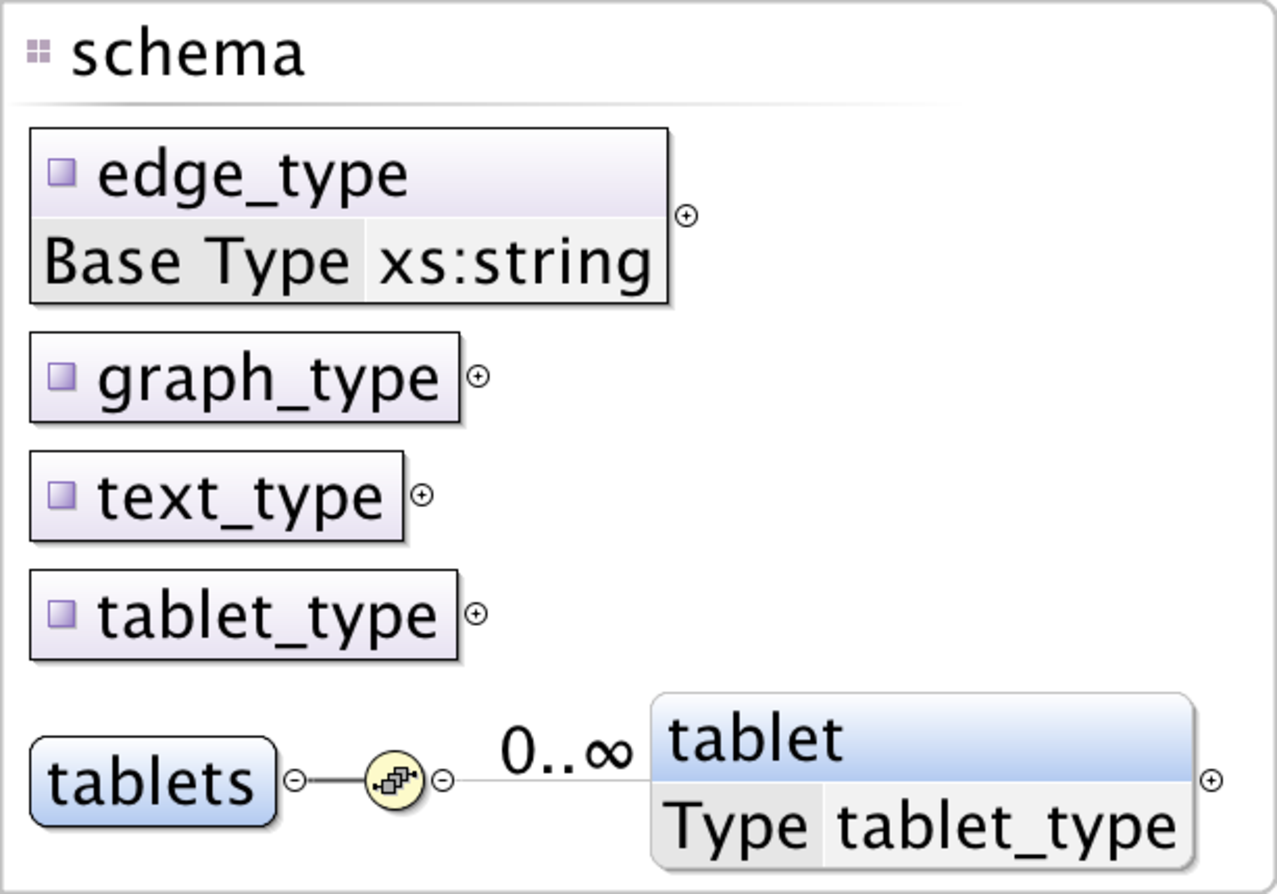
\includegraphics[width=120px]{../diagramy/schema_tablets.pdf}
 }
 \caption[Schematy poszczególnych elementów XML]{Schematy poszczególnych elementów XML\\ \footnotesize{kolor pomarańczowy oznacza atrybuty, a niebieski elementy}}
\end{figure}



Schemat dokumentu zamieszczony powyżej jest graficznym przedstawieniem dokumentu XML Schema (dodatek) 
wygenerowanym przez program Oxygen.

Jest on oparty, podobnie jak w bazie PostgreSQL, na pomyśle dra Wojciecha Jaworskiego, 
 aby przedstawić treść tabliczki w formie grafu. 
Każda krawędź tego grafu (odpowiadająca odczytowi) jest oddzielnym elementem, zawierającym atrybuty \textit{node1}, \textit{node2} 
i \textit{symbol}.
Atrybuty \textit{node1} oraz \textit{node2} oznaczają numery węzłów grafu,
natomiast atrybut \textit{symbol} to typ symbolu znajdującego się na danej krawędzi. 
Dodatkowo przechowujemy treść tabliczki w formie napisu (element \textit{show}). 

Metadane tabliczek przechowywane są w postaci podelementów elementu \textit{tablet}.


\subsubsection{Translator\_xml}
Do przeszukiwania dokumentu XML wykorzystywany jest język XQuery, będący częścią rekomendacji W3C dotyczącej XML.\\
Proste zapytanie TQL jest tłumaczone na pojedynczą konstrukcję FLWOR (For Let Where Order by Return).\\

\paragraph{Stałe fragmenty zapytania}
Każde zapytanie w części For zawiera:
	\begin{verbatim}
	FOR $tablet IN .//tablet
\end{verbatim}
a w części Return:
  \begin{verbatim}RETURN <tablet>
		{$tablet/idCDLI}
		{$tablet/publication}
		{$tablet/provenience}
		{$tablet/period}
		{$tablet/measurements}
		{$tablet/genre}
		{$tablet/subgenre}
		{$tablet/collection}
		{$tablet/museum}
		{$tablet/text/show}
		<seq>...</seq>
	</tablet>
\end{verbatim}
Zawartość elementu seq zależy od ilości sekwencji, po których wyszukujemy. 

\paragraph{Tłumaczenie zapytań o atrybuty tabliczki}

\begin{longtable}{|p{2.5in}|p{3.5in}|}
\hline
{\bf Konstrukcja} & {\bf Tłumaczenie na XQuery}\\
\hline
\endhead
provenience: wartosc & \begin{verbatim}fn:matches($tablet/provenience,'^wartosc$')\end{verbatim}
\\
\hline
publication: wartosc & \begin{verbatim}fn:matches($tablet/publication,'^wartosc$')\end{verbatim}
\\
\hline
period: wartosc & \begin{verbatim}fn:matches($tablet/period,'^wartosc$')\end{verbatim}
\\
\hline
genre: wartosc & \begin{verbatim}(fn:matches($tablet/genre,'^wartosc$')
or fn:matches($tablet/subgenre,'^wartosc$'))\end{verbatim}
\\
\hline
cdli\_id: wartosc & \begin{verbatim}fn:matches($tablet/idCDLI,'^wartosc$')\end{verbatim}
\\
\hline
\end{longtable}


\paragraph{Tłumaczenie zapytań o treść tabliczki}
Każda sekwencja, po której wyszukujemy, powoduje dodanie do zapytania następujących konstrukcji:
\begin{itemize}
\item{do części Let:}
\begin{verbatim}
let $seq <id_sekw> := (
	for $edge_end in $tablet//edge
	for $edge_start in $tablet//edge
	where (
		fn:matches($edge_start,'^<sekw[0]>$')
		and (
			some $edge1 in $tablet//edge[@node1=$edge_start/@node2]
satisfies (fn:matches($edge1,'^<sekw[1]>$')
and ... 
and fn:matches($edge_end,'^<sekw[dl_sekw-1]>$')))))
return <seq<id_sekw>> {$edge_start/@node1} {$edge_end/@node2} </seq<id_sekw>>
\end{verbatim}
\item{do części Where}
\begin{verbatim}
$seq<id_sekw>
\end{verbatim}
\item{do części Return w elemecie seq}
\begin{verbatim}
$seq<id_sekw>
\end{verbatim}
\end{itemize}




\paragraph{Tłumaczenie operatorów}
Poniższe tłumaczenia dotyczą zarówno konstrukcji prostych, jak i złożonych.

\begin{longtable}{|p{1in}|p{3in}|}
\hline
{\bf Operator} & {\bf Tłumaczenie}\\
\hline
\endhead
/ & \begin{verbatim}(<zapytanie1> or <zapytanie2>) \end{verbatim} \\
\hline
-- & \begin{verbatim}not (<zapytanie_negowane>) \end{verbatim}\\  
\hline
+ & \begin{verbatim}(<zapytanie1> and <zapytanie2>) \end{verbatim}\\ 
\hline
* & \begin{verbatim} .*\end{verbatim}  \\ 
\hline
\end{longtable}

\paragraph{Zapytania złożone}
Zapytanie złożone, składające się z wielu zapytań prostych tłumaczymy na sekwencję zapytań XQuery połączonych znakiem ','.

\subsubsection{Database\_xml}
Moduł \textit{Database\_xml} Odpowiada za wywołanie zapytania i zapisanie wyniku do struktury Tablets.
Jako bazę danych wykorzystujemy plik XML, określony w pliku konfiguracyjnym xml.conf. 
Do wyszukiwania wykorzystujemy procesor XQuery Zorba \cite{zorba}. 
Posiada on API m.in. do C++, które pozwala na przekazanie zapytania do bazy oraz przetworzenie wyniku.
